\chapter{Caminos más cortos}

\index{camino más corto}

Encontrar un camino más corto entre dos nodos
de un grafo
es un problema importante que tiene muchas
aplicaciones prácticas.
Por ejemplo, un problema natural relacionado con una red de carreteras
es calcular la longitud más corta posible de una ruta
entre dos ciudades, dadas las longitudes de las carreteras.

En un grafo no ponderado, la longitud de un camino es igual
al número de sus aristas, y podemos
simplemente usar la búsqueda en amplitud para encontrar
un camino más corto.
Sin embargo, en este capítulo nos centramos en
grafos ponderados
donde se necesitan algoritmos más sofisticados
para encontrar caminos más cortos.

\section{Algoritmo de Bellman–Ford}

\index{Algoritmo de Bellman–Ford}

El \key{algoritmo de Bellman–Ford}\footnote{El algoritmo lleva el nombre de
R. E. Bellman y L. R. Ford quienes lo publicaron independientemente
en 1958 y 1956, respectivamente \cite{bel58,for56a}.} encuentra
caminos más cortos desde un nodo de inicio hasta todos
los nodos del grafo.
El algoritmo puede procesar todo tipo de grafos,
siempre que el grafo no contenga un
ciclo con longitud negativa.
Si el grafo contiene un ciclo negativo,
el algoritmo puede detectarlo.

El algoritmo realiza un seguimiento de las distancias
desde el nodo de inicio hasta todos los nodos del grafo.
Inicialmente, la distancia al nodo de inicio es 0
y la distancia a todos los demás nodos es infinita.
El algoritmo reduce las distancias encontrando
aristas que acortan los caminos hasta que ya no es
posible reducir ninguna distancia.

\subsubsection{Ejemplo}

Consideremos cómo funciona el algoritmo de Bellman–Ford
en el siguiente grafo:
\begin{center}
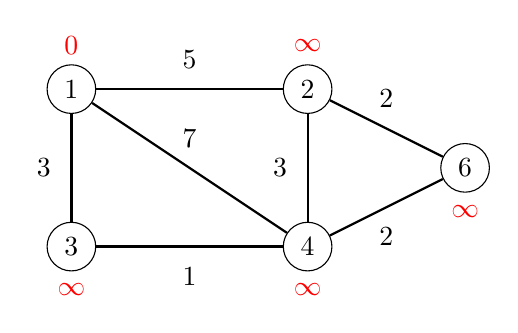
\begin{tikzpicture}
\node[draw, circle] (1) at (1,3) {1};
\node[draw, circle] (2) at (4,3) {2};
\node[draw, circle] (3) at (1,1) {3};
\node[draw, circle] (4) at (4,1) {4};
\node[draw, circle] (5) at (6,2) {6};
\node[color=red] at (1,3+0.55) {$0$};
\node[color=red] at (4,3+0.55) {$\infty$};
\node[color=red] at (1,1-0.55) {$\infty$};
\node[color=red] at (4,1-0.55) {$\infty$};
\node[color=red] at (6,2-0.55) {$\infty$};
\path[draw,thick,-] (1) -- node[font=\small,label=above:5] {} (2);
\path[draw,thick,-] (1) -- node[font=\small,label=left:3] {} (3);
\path[draw,thick,-] (3) -- node[font=\small,label=below:1] {} (4);
\path[draw,thick,-] (2) -- node[font=\small,label=left:3] {} (4);
\path[draw,thick,-] (2) -- node[font=\small,label=above:2] {} (5);
\path[draw,thick,-] (4) -- node[font=\small,label=below:2] {} (5);
\path[draw,thick,-] (1) -- node[font=\small,label=above:7] {} (4);
\end{tikzpicture}
\end{center}
A cada nodo del grafo se le asigna una distancia.
Inicialmente, la distancia al nodo de inicio es 0,
y la distancia a todos los demás nodos es infinita.

El algoritmo busca aristas que reduzcan distancias.
Primero, todas las aristas desde el nodo 1 reducen distancias:
\begin{center}
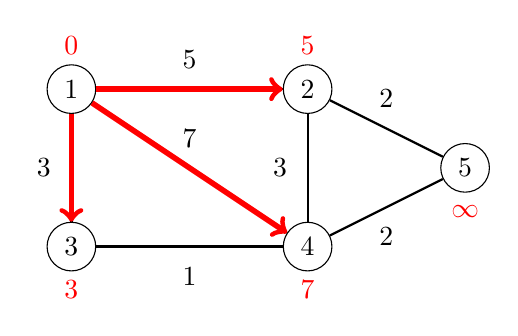
\begin{tikzpicture}
\node[draw, circle] (1) at (1,3) {1};
\node[draw, circle] (2) at (4,3) {2};
\node[draw, circle] (3) at (1,1) {3};
\node[draw, circle] (4) at (4,1) {4};
\node[draw, circle] (5) at (6,2) {5};
\node[color=red] at (1,3+0.55) {$0$};
\node[color=red] at (4,3+0.55) {$5$};
\node[color=red] at (1,1-0.55) {$3$};
\node[color=red] at (4,1-0.55) {$7$};
\node[color=red] at (6,2-0.55) {$\infty$};
\path[draw,thick,-] (1) -- node[font=\small,label=above:5] {} (2);
\path[draw,thick,-] (1) -- node[font=\small,label=left:3] {} (3);
\path[draw,thick,-] (3) -- node[font=\small,label=below:1] {} (4);
\path[draw,thick,-] (2) -- node[font=\small,label=left:3] {} (4);
\path[draw,thick,-] (2) -- node[font=\small,label=above:2] {} (5);
\path[draw,thick,-] (4) -- node[font=\small,label=below:2] {} (5);
\path[draw,thick,-] (1) -- node[font=\small,label=above:7] {} (4);

\path[draw=red,thick,->,line width=2pt] (1) -- (2);
\path[draw=red,thick,->,line width=2pt] (1) -- (3);
\path[draw=red,thick,->,line width=2pt] (1) -- (4);
\end{tikzpicture}
\end{center}
Después de esto, las aristas
$2 \rightarrow 5$ y $3 \rightarrow 4$
reducen distancias:
\begin{center}
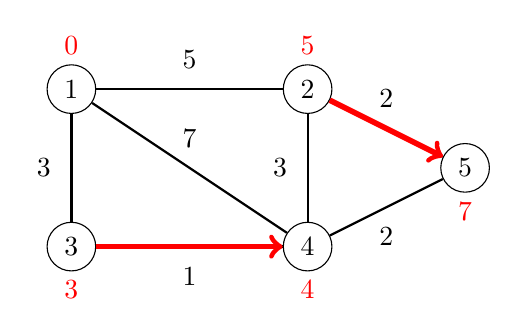
\begin{tikzpicture}
\node[draw, circle] (1) at (1,3) {1};
\node[draw, circle] (2) at (4,3) {2};
\node[draw, circle] (3) at (1,1) {3};
\node[draw, circle] (4) at (4,1) {4};
\node[draw, circle] (5) at (6,2) {5};
\node[color=red] at (1,3+0.55) {$0$};
\node[color=red] at (4,3+0.55) {$5$};
\node[color=red] at (1,1-0.55) {$3$};
\node[color=red] at (4,1-0.55) {$4$};
\node[color=red] at (6,2-0.55) {$7$};
\path[draw,thick,-] (1) -- node[font=\small,label=above:5] {} (2);
\path[draw,thick,-] (1) -- node[font=\small,label=left:3] {} (3);
\path[draw,thick,-] (3) -- node[font=\small,label=below:1] {} (4);
\path[draw,thick,-] (2) -- node[font=\small,label=left:3] {} (4);
\path[draw,thick,-] (2) -- node[font=\small,label=above:2] {} (5);
\path[draw,thick,-] (4) -- node[font=\small,label=below:2] {} (5);
\path[draw,thick,-] (1) -- node[font=\small,label=above:7] {} (4);

\path[draw=red,thick,->,line width=2pt] (2) -- (5);
\path[draw=red,thick,->,line width=2pt] (3) -- (4);
\end{tikzpicture}
\end{center}
Finalmente, hay un cambio más:
\begin{center}
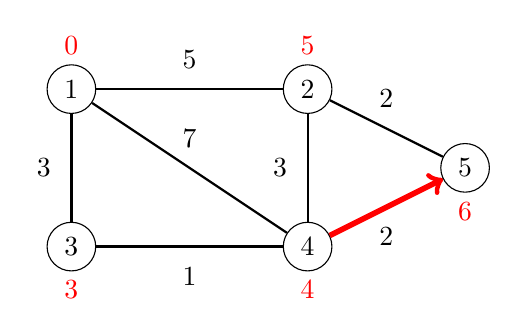
\begin{tikzpicture}
\node[draw, circle] (1) at (1,3) {1};
\node[draw, circle] (2) at (4,3) {2};
\node[draw, circle] (3) at (1,1) {3};
\node[draw, circle] (4) at (4,1) {4};
\node[draw, circle] (5) at (6,2) {5};
\node[color=red] at (1,3+0.55) {$0$};
\node[color=red] at (4,3+0.55) {$5$};
\node[color=red] at (1,1-0.55) {$3$};
\node[color=red] at (4,1-0.55) {$4$};
\node[color=red] at (6,2-0.55) {$6$};
\path[draw,thick,-] (1) -- node[font=\small,label=above:5] {} (2);
\path[draw,thick,-] (1) -- node[font=\small,label=left:3] {} (3);
\path[draw,thick,-] (3) -- node[font=\small,label=below:1] {} (4);
\path[draw,thick,-] (2) -- node[font=\small,label=left:3] {} (4);
\path[draw,thick,-] (2) -- node[font=\small,label=above:2] {} (5);
\path[draw,thick,-] (4) -- node[font=\small,label=below:2] {} (5);
\path[draw,thick,-] (1) -- node[font=\small,label=above:7] {} (4);

\path[draw=red,thick,->,line width=2pt] (4) -- (5);
\end{tikzpicture}
\end{center}

Después de esto, ninguna arista puede reducir ninguna distancia.
Esto significa que las distancias son finales,
y hemos calculado exitosamente
las distancias más cortas
desde el nodo inicial a todos los nodos del grafo.

Por ejemplo, la distancia más corta 3
desde el nodo 1 al nodo 5 corresponde a
la siguiente ruta:

\begin{center}
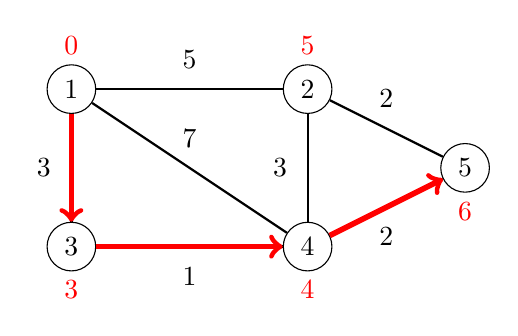
\begin{tikzpicture}
\node[draw, circle] (1) at (1,3) {1};
\node[draw, circle] (2) at (4,3) {2};
\node[draw, circle] (3) at (1,1) {3};
\node[draw, circle] (4) at (4,1) {4};
\node[draw, circle] (5) at (6,2) {5};
\node[color=red] at (1,3+0.55) {$0$};
\node[color=red] at (4,3+0.55) {$5$};
\node[color=red] at (1,1-0.55) {$3$};
\node[color=red] at (4,1-0.55) {$4$};
\node[color=red] at (6,2-0.55) {$6$};
\path[draw,thick,-] (1) -- node[font=\small,label=above:5] {} (2);
\path[draw,thick,-] (1) -- node[font=\small,label=left:3] {} (3);
\path[draw,thick,-] (3) -- node[font=\small,label=below:1] {} (4);
\path[draw,thick,-] (2) -- node[font=\small,label=left:3] {} (4);
\path[draw,thick,-] (2) -- node[font=\small,label=above:2] {} (5);
\path[draw,thick,-] (4) -- node[font=\small,label=below:2] {} (5);
\path[draw,thick,-] (1) -- node[font=\small,label=above:7] {} (4);

\path[draw=red,thick,->,line width=2pt] (1) -- (3);
\path[draw=red,thick,->,line width=2pt] (3) -- (4);
\path[draw=red,thick,->,line width=2pt] (4) -- (5);
\end{tikzpicture}
\end{center}

\subsubsection{Implementación}

La siguiente implementación del
algoritmo de Bellman–Ford determina las distancias más cortas
desde un nodo $x$ a todos los nodos del grafo.
El código asume que el grafo está almacenado
como una lista de aristas \texttt{edges}
que consiste en tuplas de la forma $(a,b,w)$,
lo que significa que hay una arista desde el nodo $a$ al nodo $b$
con peso $w$.

El algoritmo consta de $n-1$ rondas,
y en cada ronda el algoritmo recorre
todas las aristas del grafo e intenta
reducir las distancias.
El algoritmo construye una matriz \texttt{distance}
que contendrá las distancias desde $x$
a todos los nodos del grafo.
La constante \texttt{INF} denota una distancia infinita.

\begin{lstlisting}
for (int i = 1; i <= n; i++) distance[i] = INF;
distance[x] = 0;
for (int i = 1; i <= n-1; i++) {
    for (auto e : edges) {
        int a, b, w;
        tie(a, b, w) = e;
        distance[b] = min(distance[b], distance[a]+w);
    }
}
\end{lstlisting}

La complejidad temporal del algoritmo es $O(nm)$,
porque el algoritmo consta de $n-1$ rondas y
itera a través de todas las $m$ aristas durante una ronda.
Si no hay ciclos negativos en el grafo,
todas las distancias son finales después de $n-1$ rondas,
porque cada ruta más corta puede contener como máximo $n-1$ aristas.

En la práctica, las distancias finales generalmente
se pueden encontrar más rápido que en $n-1$ rondas.
Por lo tanto, una forma posible de hacer que el algoritmo sea más eficiente
es detener el algoritmo si ninguna distancia
se puede reducir durante una ronda.

\subsubsection{Ciclos negativos}

\index{ciclo negativo}

El algoritmo de Bellman–Ford también se puede usar para
comprobar si el grafo contiene un ciclo con longitud negativa.
Por ejemplo, el grafo

\begin{center}
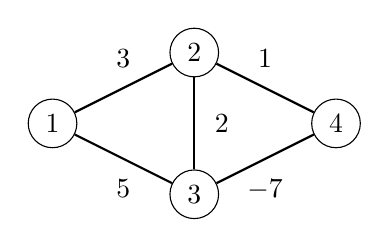
\begin{tikzpicture}[scale=0.9]
\node[draw, circle] (1) at (0,0) {$1$};
\node[draw, circle] (2) at (2,1) {$2$};
\node[draw, circle] (3) at (2,-1) {$3$};
\node[draw, circle] (4) at (4,0) {$4$};

\path[draw,thick,-] (1) -- node[font=\small,label=above:$3$] {} (2);
\path[draw,thick,-] (2) -- node[font=\small,label=above:$1$] {} (4);
\path[draw,thick,-] (1) -- node[font=\small,label=below:$5$] {} (3);
\path[draw,thick,-] (3) -- node[font=\small,label=below:$-7$] {} (4);
\path[draw,thick,-] (2) -- node[font=\small,label=right:$2$] {} (3);
\end{tikzpicture}
\end{center}
\noindent
contiene un ciclo negativo
$2 \rightarrow 3 \rightarrow 4 \rightarrow 2$
con longitud $-4$.



Si el grafo contiene un ciclo negativo,
podemos acortar infinitamente muchas veces
cualquier camino que contenga el ciclo repitiendo el ciclo
una y otra vez.
Por lo tanto, el concepto de camino más corto
no tiene sentido en esta situación.

Un ciclo negativo se puede detectar
utilizando el algoritmo de Bellman–Ford mediante
la ejecución del algoritmo durante $n$ rondas.
Si la última ronda reduce cualquier distancia,
el grafo contiene un ciclo negativo.
Tenga en cuenta que este algoritmo se puede usar para
buscar
un ciclo negativo en todo el grafo
independientemente del nodo de inicio.

\subsubsection{Algoritmo SPFA}

\index{Algoritmo SPFA}

El \key{algoritmo SPFA} (''Shortest Path Faster Algorithm'') \cite{fan94}
es una variante del algoritmo de Bellman–Ford,
que a menudo es más eficiente que el algoritmo original.
El algoritmo SPFA no recorre todos los bordes en cada ronda,
sino que, en cambio, elige los bordes que se examinarán
de una manera más inteligente.

El algoritmo mantiene una cola de nodos que podrían
usarse para reducir las distancias.
Primero, el algoritmo agrega el nodo de inicio $x$
a la cola.
Luego, el algoritmo siempre procesa el
primer nodo en la cola, y cuando un borde
$a \rightarrow b$ reduce una distancia,
el nodo $b$ se agrega a la cola.
% 
% La siguiente implementación utiliza una 
% \texttt{cola} \texttt{q}.
% Además, una matriz \texttt{inqueue} indica
% si un nodo ya está en la cola,
% en cuyo caso el algoritmo no agrega
% el nodo a la cola de nuevo.
% 
% \begin{lstlisting}
% for (int i = 1; i <= n; i++) distance[i] = INF;
% distance[x] = 0;
% q.push(x);
% while (!q.empty()) {
%     int a = q.front(); q.pop();
%     inqueue[a] = false;
%     for (auto b : v[a]) {
%         if (distance[a]+b.second < distance[b.first]) {
%             distance[b.first] = distance[a]+b.second;
%             if (!inqueue[b]) {q.push(b); inqueue[b] = true;}
%         }
%     }
% }
% \end{lstlisting}

La eficiencia del algoritmo SPFA depende
de la estructura del grafo:
el algoritmo suele ser eficiente,
pero su complejidad temporal en el peor de los casos sigue siendo
$O(nm)$ y es posible crear entradas
que hagan que el algoritmo sea tan lento como el
algoritmo original de Bellman–Ford.

\section{Algoritmo de Dijkstra}

\index{Algoritmo de Dijkstra}

El \key{algoritmo de Dijkstra}\footnote{E. W. Dijkstra publicó el algoritmo en 1959 \cite{dij59};
sin embargo, su documento original no menciona cómo implementar el algoritmo de manera eficiente.}
encuentra los caminos más cortos
desde el nodo de inicio hasta todos los nodos del grafo,
como el algoritmo de Bellman–Ford.
La ventaja del algoritmo de Dijsktra es que
es más eficiente y se puede usar para
procesar grafos grandes.
Sin embargo, el algoritmo requiere que haya
bordes sin peso negativo en el grafo.

Al igual que el algoritmo de Bellman–Ford,
el algoritmo de Dijkstra mantiene las distancias
a los nodos y las reduce durante la búsqueda.
El algoritmo de Dijkstra es eficiente porque
solo procesa
cada borde en el grafo una vez, utilizando el hecho
de que no hay bordes negativos.

\subsubsection{Ejemplo}

Consideremos cómo funciona el algoritmo de Dijkstra
en el siguiente grafo cuando el
nodo de inicio es el nodo 1:
\begin{center}
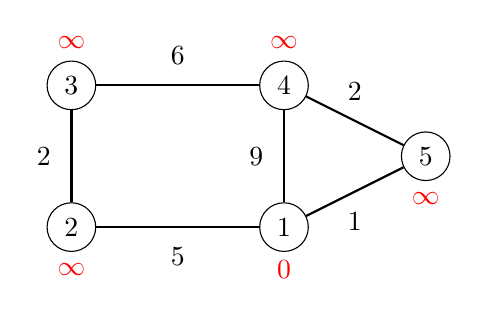
\begin{tikzpicture}[scale=0.9]
\node[draw, circle] (1) at (1,3) {3};
\node[draw, circle] (2) at (4,3) {4};
\node[draw, circle] (3) at (1,1) {2};
\node[draw, circle] (4) at (4,1) {1};
\node[draw, circle] (5) at (6,2) {5};

\node[color=red] at (1,3+0.6) {$\infty$};
\node[color=red] at (4,3+0.6) {$\infty$};
\node[color=red] at (1,1-0.6) {$\infty$};
\node[color=red] at (4,1-0.6) {$0$};
\node[color=red] at (6,2-0.6) {$\infty$};

\path[draw,thick,-] (1) -- node[font=\small,label=above:6] {} (2);
\path[draw,thick,-] (1) -- node[font=\small,label=left:2] {} (3);
\path[draw,thick,-] (3) -- node[font=\small,label=below:5] {} (4);
\path[draw,thick,-] (2) -- node[font=\small,label=left:9] {} (4);
\path[draw,thick,-] (2) -- node[font=\small,label=above:2] {} (5);
\path[draw,thick,-] (4) -- node[font=\small,label=below:1] {} (5);
\end{tikzpicture}
\end{center}
Al igual que en el algoritmo de Bellman–Ford,
inicialmente la distancia al nodo de inicio es 0
y la distancia a todos los demás nodos es infinita.

En cada paso, el algoritmo de Dijkstra selecciona un nodo
que aún no se ha procesado y cuya distancia
es lo más pequeña posible.
El primer nodo de este tipo es el nodo 1 con distancia 0.

Cuando se selecciona un nodo, el algoritmo
recorre todos los bordes que comienzan en el nodo
y reduce las distancias usándolos:
\begin{center}
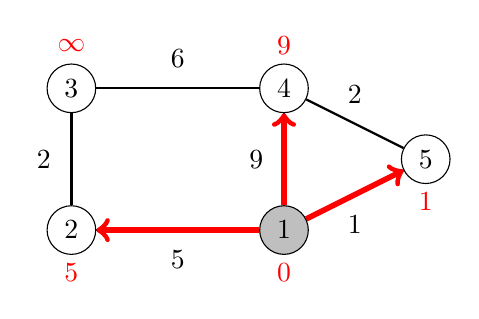
\begin{tikzpicture}[scale=0.9]
\node[draw, circle] (1) at (1,3) {3};
\node[draw, circle] (2) at (4,3) {4};
\node[draw, circle] (3) at (1,1) {2};
\node[draw, circle, fill=lightgray] (4) at (4,1) {1};
\node[draw, circle] (5) at (6,2) {5};

\node[color=red] at (1,3+0.6) {$\infty$};
\node[color=red] at (4,3+0.6) {$9$};
\node[color=red] at (1,1-0.6) {$5$};
\node[color=red] at (4,1-0.6) {$0$};
\node[color=red] at (6,2-0.6) {$1$};

\path[draw,thick,-] (1) -- node[font=\small,label=above:6] {} (2);
\path[draw,thick,-] (1) -- node[font=\small,label=left:2] {} (3);
\path[draw,thick,-] (3) -- node[font=\small,label=below:5] {} (4);
\path[draw,thick,-] (2) -- node[font=\small,label=left:9] {} (4);
\path[draw,thick,-] (2) -- node[font=\small,label=above:2] {} (5);
\path[draw,thick,-] (4) -- node[font=\small,label=below:1] {} (5);

\path[draw=red,thick,->,line width=2pt] (4) -- (2);
\path[draw=red,thick,->,line width=2pt] (4) -- (3);
\path[draw=red,thick,->,line width=2pt] (4) -- (5);
\end{tikzpicture}
\end{center}
En este caso,
los bordes del nodo 1 redujeron las distancias de
los nodos 2, 4 y 5, cuyas distancias ahora son 5, 9 y 1.

El siguiente nodo que se procesará es el nodo 5 con distancia 1.
Esto reduce la distancia al nodo 4 de 9 a 3:
\begin{center}
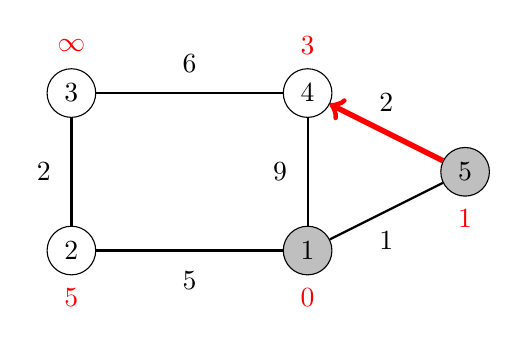
\begin{tikzpicture}
\node[draw, circle] (1) at (1,3) {3};
\node[draw, circle] (2) at (4,3) {4};
\node[draw, circle] (3) at (1,1) {2};
\node[draw, circle, fill=lightgray] (4) at (4,1) {1};
\node[draw, circle, fill=lightgray] (5) at (6,2) {5};

\node[color=red] at (1,3+0.6) {$\infty$};
\node[color=red] at (4,3+0.6) {$3$};
\node[color=red] at (1,1-0.6) {$5$};
\node[color=red] at (4,1-0.6) {$0$};
\node[color=red] at (6,2-0.6) {$1$};

\path[draw,thick,-] (1) -- node[font=\small,label=above:6] {} (2);
\path[draw,thick,-] (1) -- node[font=\small,label=left:2] {} (3);
\path[draw,thick,-] (3) -- node[font=\small,label=below:5] {} (4);
\path[draw,thick,-] (2) -- node[font=\small,label=left:9] {} (4);
\path[draw,thick,-] (2) -- node[font=\small,label=above:2] {} (5);
\path[draw,thick,-] (4) -- node[font=\small,label=below:1] {} (5);

\path[draw=red,thick,->,line width=2pt] (5) -- (2);
\end{tikzpicture}
\end{center}
Después de esto, el siguiente nodo es el nodo 4, que reduce
la distancia al nodo 3 a 9:
\begin{center}
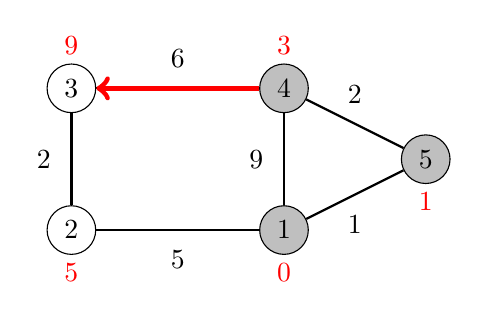
\begin{tikzpicture}[scale=0.9]
\node[draw, circle] (1) at (1,3) {3};
\node[draw, circle, fill=lightgray] (2) at (4,3) {4};
\node[draw, circle] (3) at (1,1) {2};
\node[draw, circle, fill=lightgray] (4) at (4,1) {1};
\node[draw, circle, fill=lightgray] (5) at (6,2) {5};

\node[color=red] at (1,3+0.6) {$9$};
\node[color=red] at (4,3+0.6) {$3$};
\node[color=red] at (1,1-0.6) {$5$};
\node[color=red] at (4,1-0.6) {$0$};
\node[color=red] at (6,2-0.6) {$1$};

\path[draw,thick,-] (1) -- node[font=\small,label=above:6] {} (2);
\path[draw,thick,-] (1) -- node[font=\small,label=left:2] {} (3);
\path[draw,thick,-] (3) -- node[font=\small,label=below:5] {} (4);
\path[draw,thick,-] (2) -- node[font=\small,label=left:9] {} (4);
\path[draw,thick,-] (2) -- node[font=\small,label=above:2] {} (5);
\path[draw,thick,-] (4) -- node[font=\small,label=below:1] {} (5);

\path[draw=red,thick,->,line width=2pt] (2) -- (1);
\end{tikzpicture}
\end{center}

Una propiedad notable en el algoritmo de Dijkstra es que
cada vez que se selecciona un nodo, su distancia es final.
Por ejemplo, en este punto del algoritmo,
las distancias 0, 1 y 3 son las distancias finales
a los nodos 1, 5 y 4.

Después de esto, el algoritmo procesa los dos
nodos restantes, y las distancias finales son las siguientes:

\begin{center}
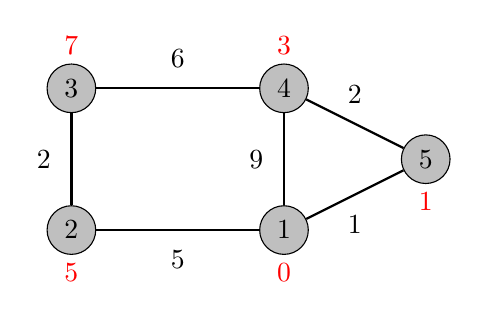
\begin{tikzpicture}[scale=0.9]
\node[draw, circle, fill=lightgray] (1) at (1,3) {3};
\node[draw, circle, fill=lightgray] (2) at (4,3) {4};
\node[draw, circle, fill=lightgray] (3) at (1,1) {2};
\node[draw, circle, fill=lightgray] (4) at (4,1) {1};
\node[draw, circle, fill=lightgray] (5) at (6,2) {5};

\node[color=red] at (1,3+0.6) {$7$};
\node[color=red] at (4,3+0.6) {$3$};
\node[color=red] at (1,1-0.6) {$5$};
\node[color=red] at (4,1-0.6) {$0$};
\node[color=red] at (6,2-0.6) {$1$};

\path[draw,thick,-] (1) -- node[font=\small,label=above:6] {} (2);
\path[draw,thick,-] (1) -- node[font=\small,label=left:2] {} (3);
\path[draw,thick,-] (3) -- node[font=\small,label=below:5] {} (4);
\path[draw,thick,-] (2) -- node[font=\small,label=left:9] {} (4);
\path[draw,thick,-] (2) -- node[font=\small,label=above:2] {} (5);
\path[draw,thick,-] (4) -- node[font=\small,label=below:1] {} (5);
\end{tikzpicture}
\end{center}

\subsubsection{Aristas negativas}

La eficiencia del algoritmo de Dijkstra es
basada en el hecho de que el gráfico no
contiene aristas negativas.
Si hay una arista negativa,
el algoritmo puede dar resultados incorrectos.
Como ejemplo, considere el siguiente gráfico:

\begin{center}
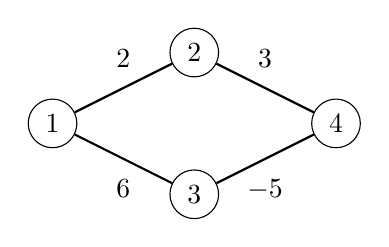
\begin{tikzpicture}[scale=0.9]
\node[draw, circle] (1) at (0,0) {$1$};
\node[draw, circle] (2) at (2,1) {$2$};
\node[draw, circle] (3) at (2,-1) {$3$};
\node[draw, circle] (4) at (4,0) {$4$};

\path[draw,thick,-] (1) -- node[font=\small,label=above:2] {} (2);
\path[draw,thick,-] (2) -- node[font=\small,label=above:3] {} (4);
\path[draw,thick,-] (1) -- node[font=\small,label=below:6] {} (3);
\path[draw,thick,-] (3) -- node[font=\small,label=below:$-5$] {} (4);
\end{tikzpicture}
\end{center}
\noindent
El camino más corto desde el nodo 1 hasta el nodo 4 es
$1 \rightarrow 3 \rightarrow 4$
y su longitud es 1.
Sin embargo, el algoritmo de Dijkstra
encuentra el camino $1 \rightarrow 2 \rightarrow 4$
siguiendo las aristas de peso mínimo.
El algoritmo no tiene en cuenta que
en el otro camino, el peso $-5$
compensa el peso anterior grande $6$.

\subsubsection{Implementación}

La siguiente implementación del algoritmo de Dijkstra
calcula las distancias mínimas desde un nodo $x$
a otros nodos del gráfico.
El gráfico se almacena como listas de adyacencia
de modo que \texttt{adj[$a$]} contiene un par $(b,w)$
siempre que haya una arista desde el nodo $a$ hasta el nodo $b$
con peso $w$.

Una implementación eficiente del algoritmo de Dijkstra
requiere que sea posible encontrar eficientemente el
nodo de distancia mínima que no se ha procesado.
Una estructura de datos apropiada para esto es una cola de prioridad
que contiene los nodos ordenados por sus distancias.
Usando una cola de prioridad, el siguiente nodo a procesar
se puede recuperar en tiempo logarítmico.

En el siguiente código, la cola de prioridad
\texttt{q} contiene pares de la forma $(-d,x)$,
lo que significa que la distancia actual al nodo $x$ es $d$.
El array \texttt{distance} contiene la distancia a
cada nodo, y el array \texttt{processed} indica
si un nodo se ha procesado.
Inicialmente la distancia es $0$ a $x$ e $\infty$ a todos los demás nodos.

\begin{lstlisting}
for (int i = 1; i <= n; i++) distance[i] = INF;
distance[x] = 0;
q.push({0,x});
while (!q.empty()) {
    int a = q.top().second; q.pop();
    if (processed[a]) continue;
    processed[a] = true;
    for (auto u : adj[a]) {
        int b = u.first, w = u.second;
        if (distance[a]+w < distance[b]) {
            distance[b] = distance[a]+w;
            q.push({-distance[b],b});
        }
    }
}
\end{lstlisting}

Tenga en cuenta que la cola de prioridad contiene \emph{negativas}
distancias a los nodos.
La razón de esto es que
la versión predeterminada de la cola de prioridad de C++ encuentra el máximo
elementos, mientras que queremos encontrar elementos mínimos.
Al usar distancias negativas,
podemos usar directamente la cola de prioridad predeterminada\footnote{Por
supuesto, también podríamos declarar la cola de prioridad como en el Capítulo 4.5
y usar distancias positivas, pero la implementación sería un poco más larga.}.
También tenga en cuenta que puede haber varias instancias del mismo
nodo en la cola de prioridad; sin embargo, solo la instancia con la
distancia mínima será procesada.

La complejidad temporal de la implementación anterior es
$O(n+m \log m)$, porque el algoritmo pasa por
todos los nodos del gráfico y agrega para cada arista
como máximo una distancia a la cola de prioridad.

\section{Algoritmo de Floyd–Warshall}

\index{Algoritmo de Floyd–Warshall}

El \key{algoritmo de Floyd–Warshall}\footnote{El algoritmo
lleva el nombre de R. W. Floyd y S. Warshall
que lo publicaron de forma independiente en 1962 \cite{flo62,war62}.}
proporciona una forma alternativa de abordar el problema
de encontrar las rutas más cortas.
A diferencia de los otros algoritmos de este capítulo,
encuentra todas las rutas más cortas entre los nodos
en una sola pasada.

El algoritmo mantiene una matriz bidimensional
que contiene las distancias entre los nodos.
Primero, las distancias se calculan solo usando
aristas directas entre los nodos,
y después de esto, el algoritmo reduce las distancias
usando nodos intermedios en las rutas.

\subsubsection{Ejemplo}

Consideremos cómo funciona el algoritmo de Floyd–Warshall
en el siguiente gráfico:

\begin{center}
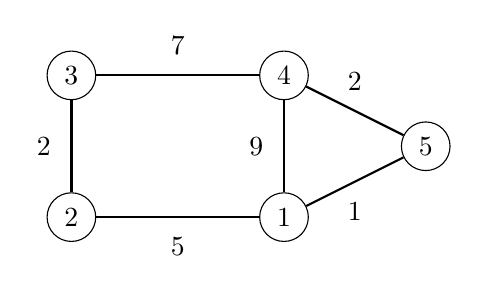
\begin{tikzpicture}[scale=0.9]
\node[draw, circle] (1) at (1,3) {$3$};
\node[draw, circle] (2) at (4,3) {$4$};
\node[draw, circle] (3) at (1,1) {$2$};
\node[draw, circle] (4) at (4,1) {$1$};
\node[draw, circle] (5) at (6,2) {$5$};

\path[draw,thick,-] (1) -- node[font=\small,label=above:7] {} (2);
\path[draw,thick,-] (1) -- node[font=\small,label=left:2] {} (3);
\path[draw,thick,-] (3) -- node[font=\small,label=below:5] {} (4);
\path[draw,thick,-] (2) -- node[font=\small,label=left:9] {} (4);
\path[draw,thick,-] (2) -- node[font=\small,label=above:2] {} (5);
\path[draw,thick,-] (4) -- node[font=\small,label=below:1] {} (5);
\end{tikzpicture}
\end{center}

Inicialmente, la distancia desde cada nodo a sí mismo es $0$,
y la distancia entre los nodos $a$ y $b$ es $x$
si hay una arista entre los nodos $a$ y $b$ con peso $x$.
Todas las demás distancias son infinitas.
En este gráfico, la matriz inicial es la siguiente:
\begin{center}
\begin{tabular}{r|rrrrr}
 & 1 & 2 & 3 & 4 & 5 \\
\hline
1 & 0 & 5 & $\infty$ & 9 & 1 \\
2 & 5 & 0 & 2 & $\infty$ & $\infty$ \\
3 & $\infty$ & 2 & 0 & 7 & $\infty$ \\
4 & 9 & $\infty$ & 7 & 0 & 2 \\
5 & 1 & $\infty$ & $\infty$ & 2 & 0 \\
\end{tabular}
\end{center}
\vspace{10pt}
El algoritmo consiste en rondas consecutivas.
En cada ronda, el algoritmo selecciona un nuevo nodo
que puede actuar como un nodo intermedio en las rutas a partir de ahora,
y las distancias se reducen usando este nodo.

En la primera ronda, el nodo 1 es el nuevo nodo intermedio.
Hay una nueva ruta entre los nodos 2 y 4
con longitud 14, porque el nodo 1 los conecta.
También hay una nueva ruta 
entre los nodos 2 y 5 con longitud 6.

\begin{center}
\begin{tabular}{r|rrrrr}
 & 1 & 2 & 3 & 4 & 5 \\
\hline
1 & 0 & 5 & $\infty$ & 9 & 1 \\
2 & 5 & 0 & 2 & \textbf{14} & \textbf{6} \\
3 & $\infty$ & 2 & 0 & 7 & $\infty$ \\
4 & 9 & \textbf{14} & 7 & 0 & 2 \\
5 & 1 & \textbf{6} & $\infty$ & 2 & 0 \\
\end{tabular}
\end{center}
\vspace{10pt}

En la segunda ronda, el nodo 2 es el nuevo nodo intermedio.
Esto crea nuevas rutas entre los nodos 1 y 3
y entre los nodos 3 y 5:

\begin{center}
\begin{tabular}{r|rrrrr}
 & 1 & 2 & 3 & 4 & 5 \\
\hline
1 & 0 & 5 & \textbf{7} & 9 & 1 \\
2 & 5 & 0 & 2 & 14 & 6 \\
3 & \textbf{7} & 2 & 0 & 7 & \textbf{8} \\
4 & 9 & 14 & 7 & 0 & 2 \\
5 & 1 & 6 & \textbf{8} & 2 & 0 \\
\end{tabular}
\end{center}
\vspace{10pt}

En la tercera ronda, el nodo 3 es el nuevo nodo intermedio.
Hay una nueva ruta entre los nodos 2 y 4:

\begin{center}
\begin{tabular}{r|rrrrr}
 & 1 & 2 & 3 & 4 & 5 \\
\hline
1 & 0 & 5 & 7 & 9 & 1 \\
2 & 5 & 0 & 2 & \textbf{9} & 6 \\
3 & 7 & 2 & 0 & 7 & 8 \\
4 & 9 & \textbf{9} & 7 & 0 & 2 \\
5 & 1 & 6 & 8 & 2 & 0 \\
\end{tabular}
\end{center}
\vspace{10pt}

El algoritmo continúa así,
hasta que todos los nodos han sido nombrados nodos intermedios.
Después de que el algoritmo ha terminado, la matriz contiene
las distancias mínimas entre dos nodos cualesquiera:

\begin{center}
\begin{tabular}{r|rrrrr}
 & 1 & 2 & 3 & 4 & 5 \\
\hline
1 & 0 & 5 & 7 & 3 & 1 \\
2 & 5 & 0 & 2 & 8 & 6 \\
3 & 7 & 2 & 0 & 7 & 8 \\
4 & 3 & 8 & 7 & 0 & 2 \\
5 & 1 & 6 & 8 & 2 & 0 \\
\end{tabular}
\end{center}

Por ejemplo, la matriz nos dice que la
distancia más corta entre los nodos 2 y 4 es 8.
Esto corresponde a la siguiente ruta:

\begin{center}
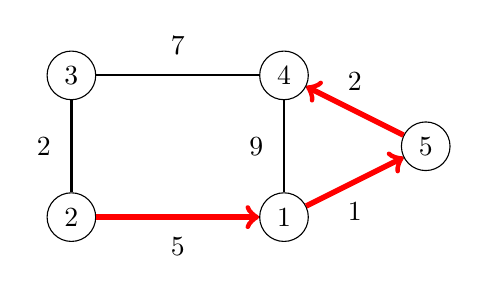
\begin{tikzpicture}[scale=0.9]
\node[draw, circle] (1) at (1,3) {$3$};
\node[draw, circle] (2) at (4,3) {$4$};
\node[draw, circle] (3) at (1,1) {$2$};
\node[draw, circle] (4) at (4,1) {$1$};
\node[draw, circle] (5) at (6,2) {$5$};

\path[draw,thick,-] (1) -- node[font=\small,label=above:7] {} (2);
\path[draw,thick,-] (1) -- node[font=\small,label=left:2] {} (3);
\path[draw,thick,-] (3) -- node[font=\small,label=below:5] {} (4);
\path[draw,thick,-] (2) -- node[font=\small,label=left:9] {} (4);
\path[draw,thick,-] (2) -- node[font=\small,label=above:2] {} (5);
\path[draw,thick,-] (4) -- node[font=\small,label=below:1] {} (5);

\path[draw=red,thick,->,line width=2pt] (3) -- (4);
\path[draw=red,thick,->,line width=2pt] (4) -- (5);
\path[draw=red,thick,->,line width=2pt] (5) -- (2);
\end{tikzpicture}
\end{center}

\subsubsection{Implementación}

La ventaja del
algoritmo de Floyd–Warshall es que es
fácil de implementar.
El siguiente código construye una
matriz de distancia donde $\texttt{distance}[a][b]$
es la distancia más corta entre los nodos $a$ y $b$.
Primero, el algoritmo inicializa \texttt{distance}
usando la matriz de adyacencia \texttt{adj} del gráfico:

\begin{lstlisting}
for (int i = 1; i <= n; i++) {
    for (int j = 1; j <= n; j++) {
        if (i == j) distance[i][j] = 0;
        else if (adj[i][j]) distance[i][j] = adj[i][j];
        else distance[i][j] = INF;
    }
}
\end{lstlisting}
Después de esto, las distancias más cortas se pueden encontrar de la siguiente manera:
\begin{lstlisting}
for (int k = 1; k <= n; k++) {
    for (int i = 1; i <= n; i++) {
        for (int j = 1; j <= n; j++) {
            distance[i][j] = min(distance[i][j],
                                   distance[i][k]+distance[k][j]);
        }
    }
}
\end{lstlisting}

La complejidad temporal del algoritmo es $O(n^3)$,
porque contiene tres bucles anidados
que recorren los nodos del gráfico.

Dado que la implementación del algoritmo de Floyd–Warshall
es simple, el algoritmo puede ser
una buena opción incluso si solo se necesita para encontrar un
solo camino más corto en el gráfico.
Sin embargo, el algoritmo solo se puede usar cuando el gráfico
es tan pequeño que una complejidad temporal cúbica es lo suficientemente rápida.
